\documentclass[aspectratio=1610,t]{beamer}

% Colors
\usepackage{color}
\definecolor{mainorange}{HTML}{EC811B}
\definecolor{lightgrey}{HTML}{888888}

% Syntax highlighting
\usepackage{minted}
\usepackage{alltt}
\newcommand\hi[1]{{\color{mainorange} \textbf{#1}}}

% Theme
\usetheme[%
    sectionpage=none,
	subsectionpage=none,
	numbering=fraction,
	progressbar=foot,
]{metropolis}

% Customization
\setbeamertemplate{section in toc}[sections numbered]
\setbeamerfont{title}{size=\fontsize{30}{30}}
\setbeamerfont{block title}{size=\large}
\newcommand\sep{\textcolor{lightgrey}{\rule{\linewidth}{0.05mm}}}

% Meta
\title{LibrePCB}
\date{\today}
\author{Urban Bruhin}
\institute{Coredump Rapperswil}

\begin{document}

\pgfdeclareimage[width=\paperwidth]{bg}{images/background-dark.pdf}
\usebackgroundtemplate{\pgfuseimage{bg}}
\maketitle

% ----------------------------------------------------------------- %

%\begin{frame}[plain,noframenumbering]
%	\frametitle{Table of Contents}
%	\setcounter{tocdepth}{1}
%	\tableofcontents
%\end{frame}

% ----------------------------------------------------------------- %

\pgfdeclareimage[width=\paperwidth]{bg}{images/background-light.pdf}
\usebackgroundtemplate{\pgfuseimage{bg}}

\section{About LibrePCB}

\begin{frame}{About LibrePCB}
  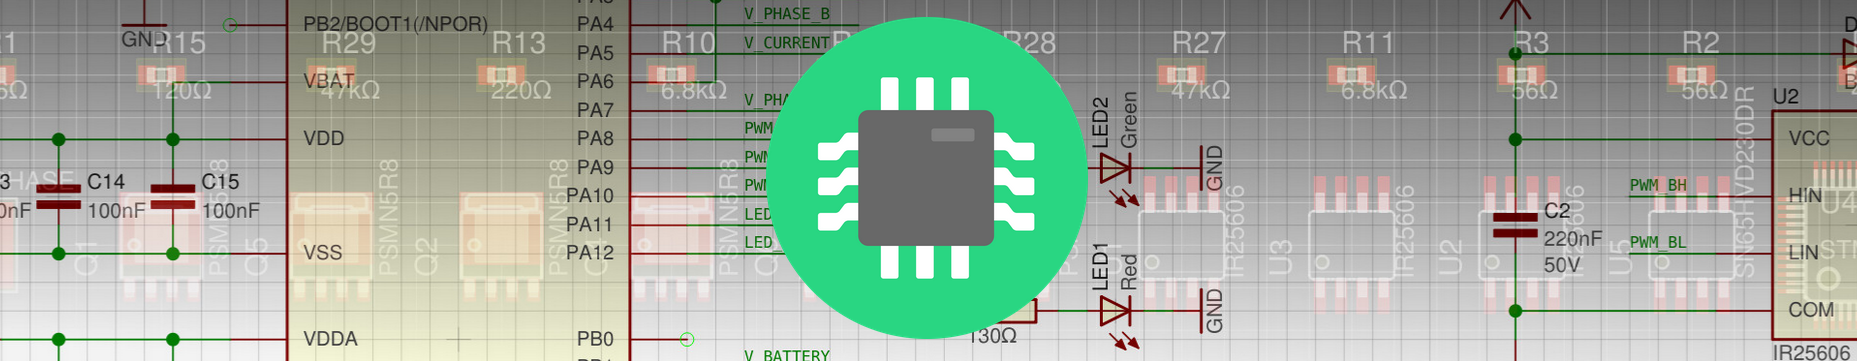
\includegraphics[width=\linewidth]{images/header.png} \linebreak\linebreak
  \textbf{Free/OpenSource EDA Software (Electronic Design Automation)}
  \begin{itemize}
    \item Multiplatform (Linux/Unix, Mac OS X, Windows)
    \item Written in C++/Qt
    \item Development started in February 2013
    \item Website: \url{http://librepcb.org/}
    \item GitHub: \url{https://github.com/LibrePCB/LibrePCB}
  \end{itemize}
\end{frame}

% ----------------------------------------------------------------- %

\section{Why LibrePCB?}

\begin{frame}{Why LibrePCB?}
  \textbf{Most EDA tools have some big issues:}
  \begin{itemize}
   	\item Only available for Windows
    \item High license costs, even for updates
    \item Free/hobby versions not allowed for commercial use
    \item Limitations in PCB size, count of schematics, pads or vias
    \item Old-fashioned, non-intuitive user interface
    \item Proprietary binary file format, not usable for version control
    \item Enforcement of cloud storage
    \item Library system unflexible and cumbersome
  \end{itemize}
\end{frame}

% ----------------------------------------------------------------- %

\section{All-In-One Application}

\begin{frame}{All-In-One Application}
	\begin{center}
		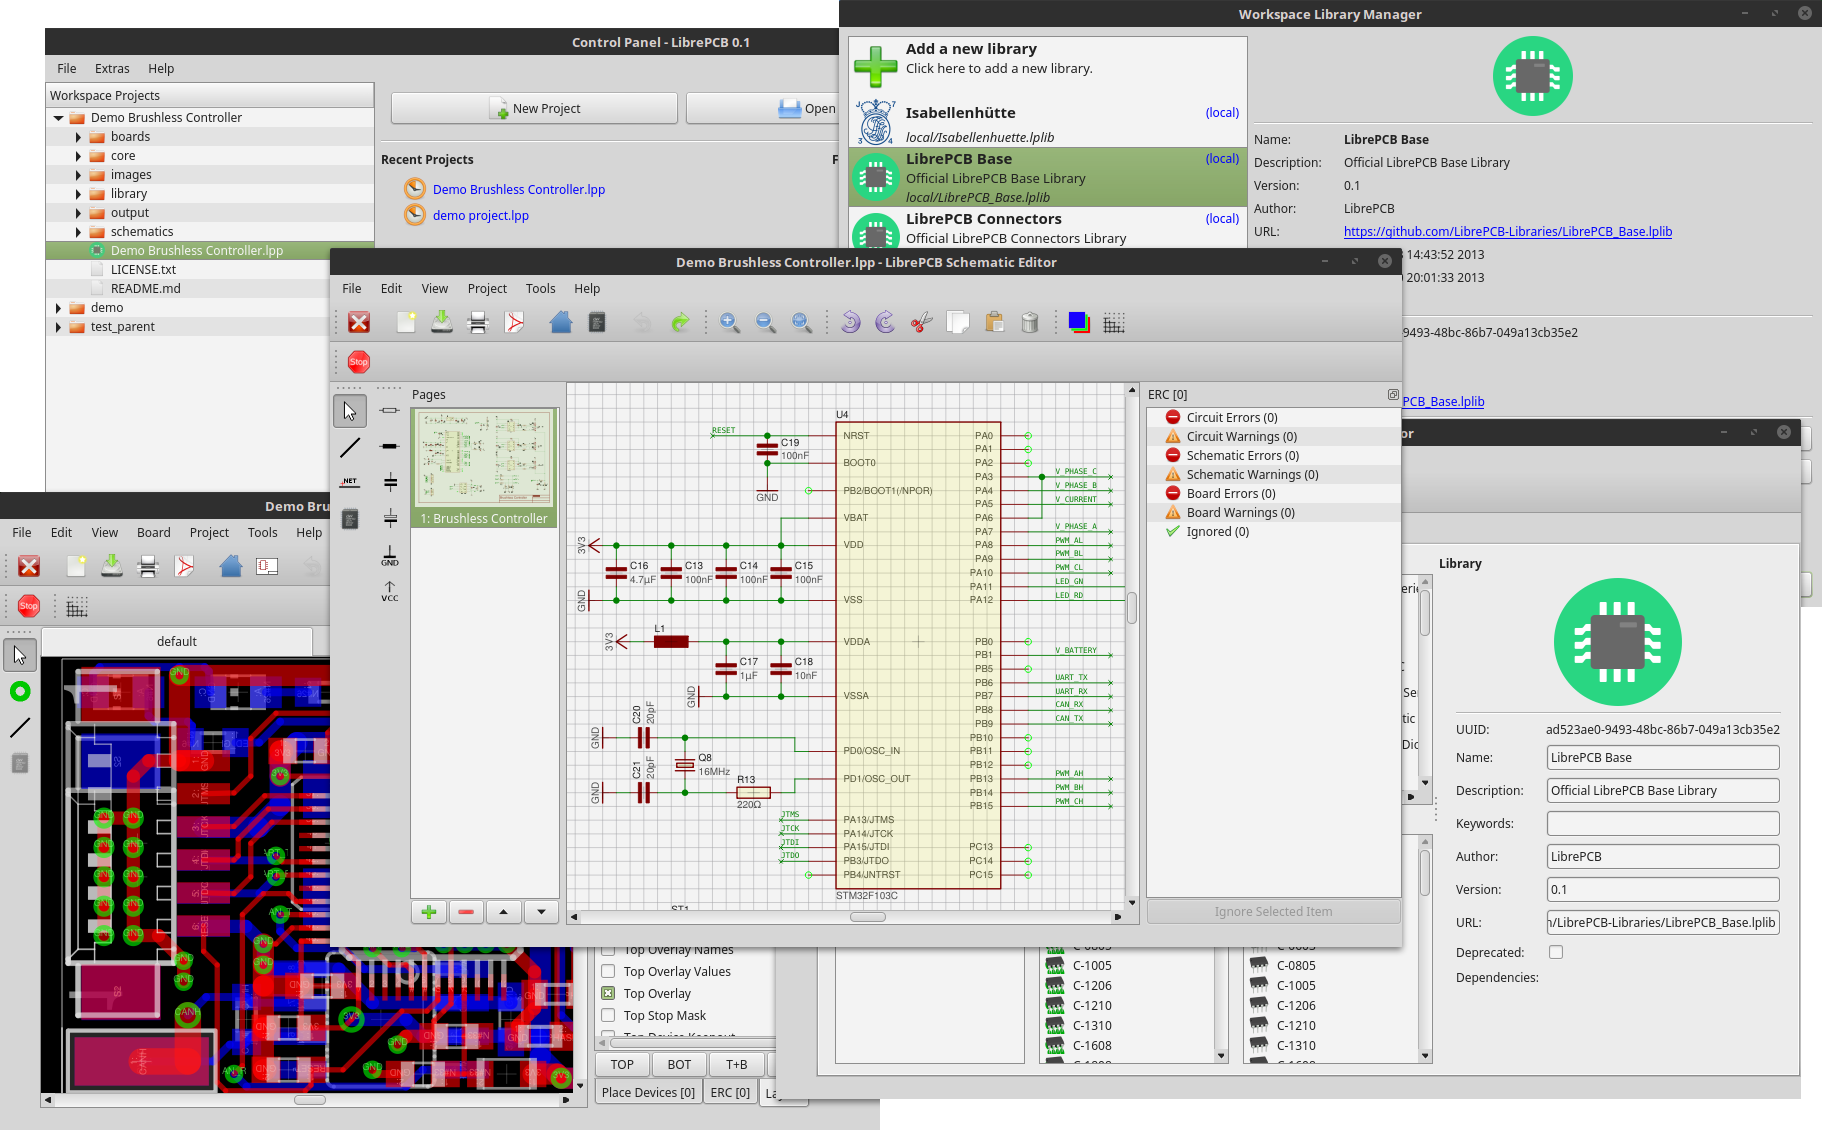
\includegraphics[width=0.8\paperwidth]{images/overview.png}
	\end{center}
\end{frame}

% ----------------------------------------------------------------- %

\section{Schematic Editor}

\begin{frame}{Schematic Editor}
	\begin{center}
		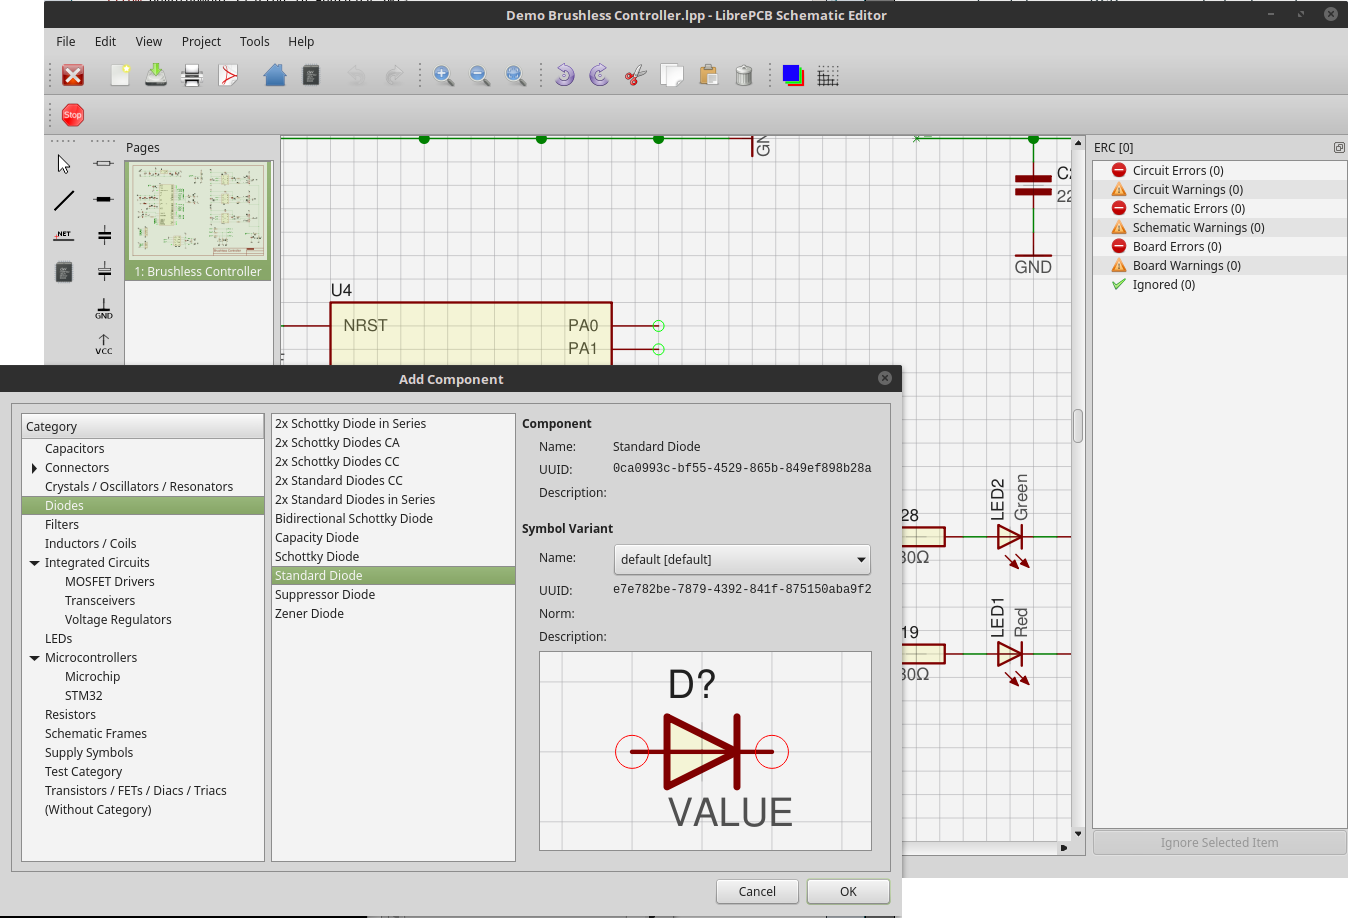
\includegraphics[width=0.7\paperwidth]{images/schematic_editor.png}
	\end{center}
\end{frame}

% ----------------------------------------------------------------- %

\section{Board Editor}

\begin{frame}{Board Editor}
	\begin{center}
		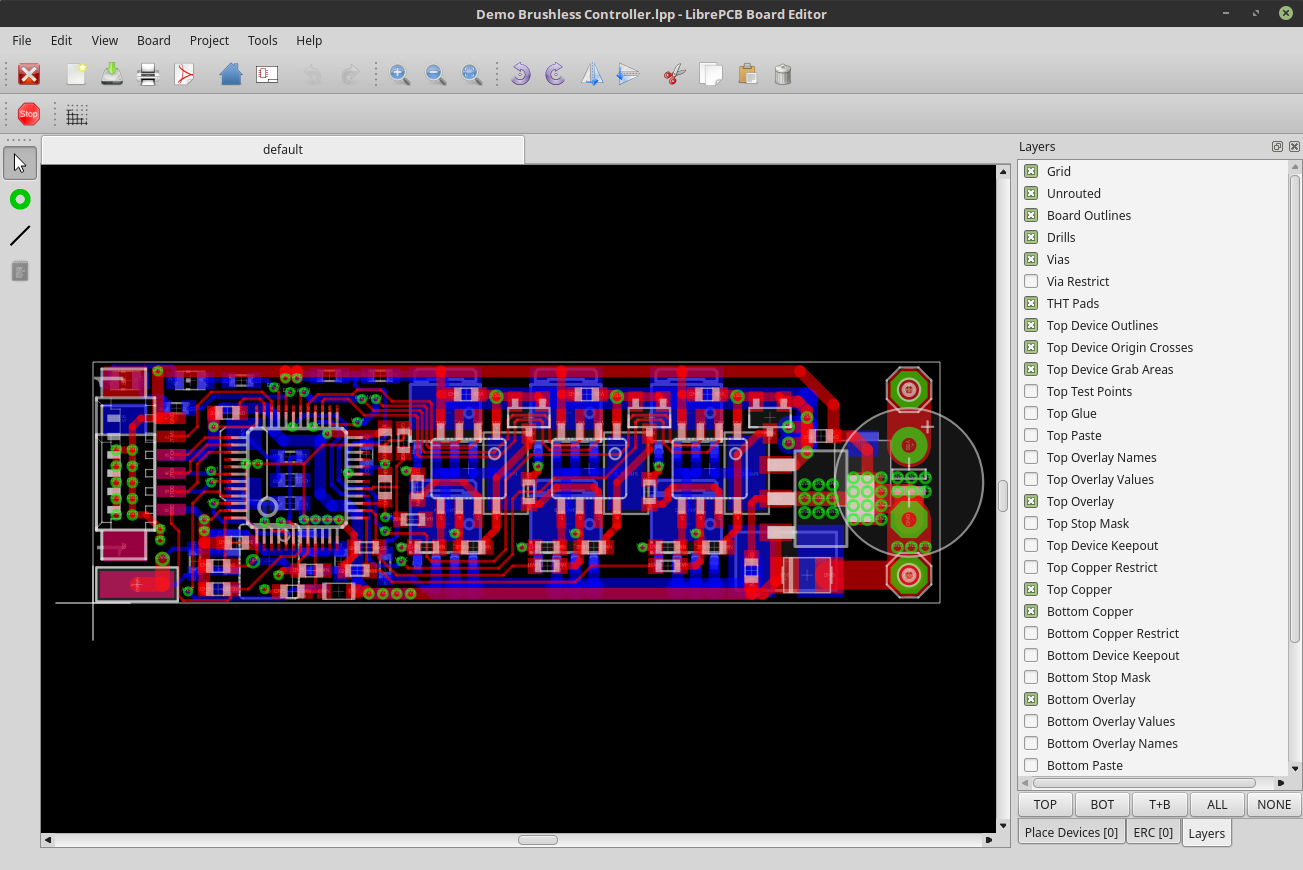
\includegraphics[width=0.7\paperwidth]{images/board_editor.png}
	\end{center}
\end{frame}

% ----------------------------------------------------------------- %

\section{Library Manager}

\begin{frame}{Library Manager}
	\begin{center}
		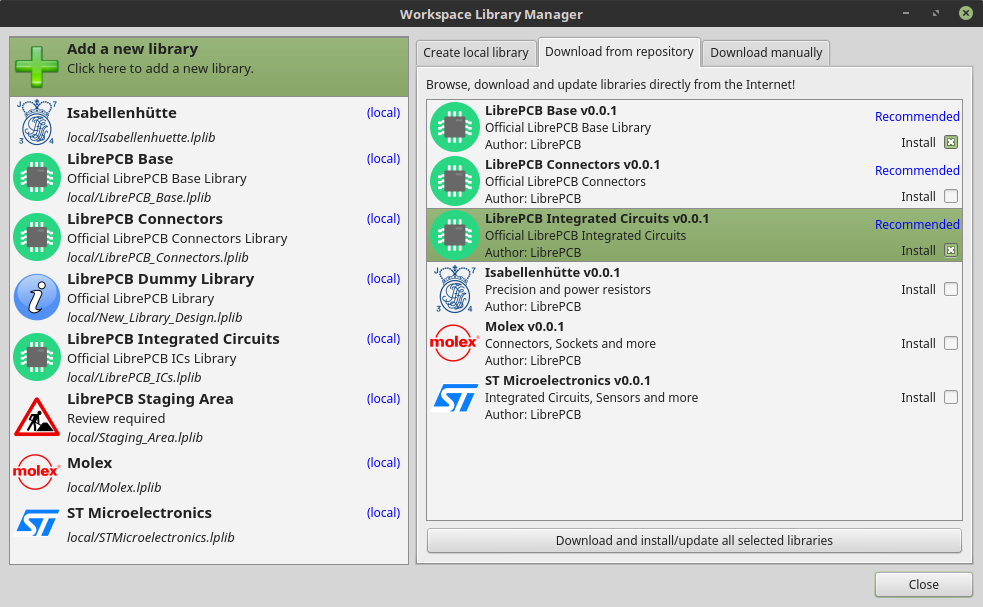
\includegraphics[width=0.7\paperwidth]{images/library_manager.png}
	\end{center}
\end{frame}

% ----------------------------------------------------------------- %

\section{Contributing}

\begin{frame}{Contributing}
  \begin{centering}
    \bigskip \bigskip
    \textbf{\Huge Contributors wanted!}\\
    \bigskip \bigskip
    \textbf{\Large Fork - Commit - Pull Request}\\
    \bigskip \bigskip
    {\small \url{https://github.com/LibrePCB/LibrePCB/blob/master/CONTRIBUTING.md}}\\
  \end{centering}
\end{frame}

% ----------------------------------------------------------------- %

{
\setbeamertemplate{footline}{}
\pgfdeclareimage[width=\paperwidth]{bg}{images/background-inverted.pdf}
\usebackgroundtemplate{\pgfuseimage{bg}}
\begin{frame}[standout]
	\begin{centering}
	{\Huge Thank you!}\\
	{\normalsize \url{www.coredump.ch}}\\
	\end{centering}
\end{frame}
}

\end{document}
